\chapter{绪论}
\label{chp:installation}


\section{研究工作的背景及意义}

城市旅行需求在过去几十年里由于人口和城市化的快速增长而急剧上升。增长速度远超过了交通基础设施的扩展。需求与供应失衡的后果就是全球范围内普遍存在的交通拥堵,这也说明了各种出行需求管理策略的出现和必要性。然而,这些策略的成功实施在很大程度上取决于如何理解和建模出行者的出行选择。为了获得准确的出行需求预测并实施有效的需求管理策略,研究人员和政府机构了解出行者在出行时如何进行决策将会至关重要。一旦决策者知道出行者在何时何地以及将采取什么模式出行,就可以提供有效的解决方案来缓解拥堵。因此,出行决策建模成为交通研究的关键。

研究人员通常将出行决策描述为不同维度的备选方案选择,例如出发时间、目的地、方式和路线。这些选择问题通常被描述为离散或者连续选择模型。早期的出行决策模型只考虑了一个维度,即从该选择维度的一组相互排斥的备选方案中选择了一个备选方案。然而在实际生活中,需要结合不同行为维度的进行多维决策才足以支持日益增长的拥堵管理策略应用。与传统的单维度出行选择模型不同,多维度模型考虑了不同选择之间的相关性。与模式和出发时间相关的两个关键且相关的选择从微观角度来看,这两个选择反映了个体对其出行的偏好。从宏观角度来看,它们决定了交通网络的时空旅行需求。我们强调,交通方式的吸引力以及其可能的选择取决于其服务水平。这种服务水平可能受到诸如拥堵定价、公共交通优先、各种类型激励等众多政策措施的影响。因此,为了评估这些政策措施,有必要建立一个同时考虑出行方式和出发时间选择的建模框架。


大多数现有的关于建模联合出行方式和出发时间选择的研究都是使用不同类型的离散选择模型(DCM),主要寻求随机效用最大化。特别是,考虑到它们在描述不同选择替代方案之间的相关性方面的能力,通常使用诸如多项式logit(MNL)、嵌套logit(NL)、交叉嵌套logit(CNL)等模型。利用随机效用最大化的模型依靠着其强大的理论依据而被广泛地应用。基于随机效用的模型是可以解释出行选择的基本理论,而对于复杂的决策过程建模的适用性,尤其是在选择预测中,可能会受到随机效用函数中线性结构的限制。对于多维选择问题,不同维度之间的关联结构也需要预先确定。尽管这些模型在理论上是解决旅行选择问题的典型解决方案,但在复杂决策过程中,由于随机效用函数的表述限制,它们的适用性可能受到限制。由于缺乏适应性以及出行者对旅行信息的不完美感知,由离散选择模型所推导出的出行选择可能不一定会导致最佳结果。

效用的随机成分不仅可以解释出行者对与观察信息的局限性,而且可以考虑决策者的不完全信息和偏好的随机变化。然而,以下事实支持了对基于学习方法的出行选择模型的需求。首先,乘客在模式选择的决策过程,是由不同出行方式的服务水平信息告知和指导的。这些知识通常是通过各种方式获得的(包括出行经验),并且会随着时间动态变化。第二,出行决策受到一些行为因素的影响,其中部分乘客更倾向于(更少)选择(改变)他们已经习惯的模式。第三,交通系统的随机性和时间依赖性最有可能引起出行者的自适应模式切换决策,在这种决策中,出行者可能会根据以往的经验更新他们对每种出行模式的预期效用。传统方法不能解决决策过程中涉及的时间维度。因此,与传统的选择建模方法相比,基于学习的出行决策模型更可取。

近年来,深度强化学习已成为应对复杂决策问题的关键机器学习方法之一,原因在于它在复杂环境中具有较强的学习能力。这种学习能力正是传统离散选择模型所缺乏的,可以充分用于出行选择建模或出行推荐。出行选择的决策过程是一个复杂的过程,会受到环境的影响而不断地变化,通过建立传统的出行选择模型来解释出行行为的方法过于理想化。而此类场景很好地契合了深度强化学习“无模型、自学习、数据驱动”,使用深度强化学习的方法可以将此类复杂的模型使 用深度神经网络进行描述,提取不同外界环境的特征数据如等待时间、出行成本等构建 状态输入,再对出行者的出行行为进行优化,利用大数据训练网络增加其真实性和可靠性。相较于传统的离散选择模型,深度强化学习的方法对复杂的场景适应能力有极大的提升,并且适用的场景更加广泛。


\section{国内外研究}

\subsection{基于随机效用的离散选择模型}
在出行选择的模型中,通常使用基于随机效用的离散选择模型对不同维度的选择行为进行建模。从McFadden\cite{mcfadden1973conditional}在 1973 年提出 Multinomial Logit(MNL)模型以来,Logit系列模型被广泛应用于出行决策问题。MNL方法解决出行方式和出发时间选择问题的原因主要是由于MNL模型具有简单、易于应用和计算效率高等特点,而且在解决出行选择问题上已被广泛应用并取得了一定的成果。刘炳恩等\cite{GLJK200805021}使用非集计离散选择模型,基于北京居民出行调查数据,建立了交通方式选择MNL模型,并通过参数标定和命中率计算验证了模型的有效性。结果表明,该方法能较全面地考虑影响因素,尤其是出行者的个人特性,提高了模型的预测精度和实用性。此外,MNL模型还具有广泛的理论基础和应用场景,能够在一定程度上满足研究者对出行选择行为进行建模的需求。CHANG等\cite{MeiShiangCHANG2013}在探讨音乐会参与者在出行方式和到达时间选择方面的行为,运用多项式Logit模型探讨了影响其出行选择的最有效因素,帮助预测在计划特殊事件中每种出行方式的时间依赖性旅行需求。然而,MNL存在一个被广泛承认的问题:它假设了不相关的替代方案之间的独立性,也称为IIA(独立不相关)特性。这意味着未被观察到的特征在不同选项之间是不相关的,然而在一些出行选择问题中,这个假设不成立。例如,在离散的出发时间选择中,相邻的出发时间区间的未观察到的特征往往表现出显著的相关性。

为了解决这一问题,NL模型\cite{train1978goods}被提出来克服IIA的限制。NL模型能够识别嵌套组内不同替代方案之间的相关性,因此能更好地描述出行者在做出选择时的现实决策过程,从而提高模型的预测精度和实用性。诸葛承祥等\cite{诸葛承祥}基于北京市居民出行调查数据,建立了两个方向的Nested Logit模型来分析通勤者的出行时间和出行方式选择特征,结果表明出行时间—出行方式选择模型比出行方式—出行时间选择模型更合理,可以为高峰时期的管理政策提供理论依据。Koppelman\cite{KOPPELMAN2005825}提出了一个基于MNL和NL模型的整合模型,通过对非独立误差、异方差和协方差异方差等方面进行拓展,使得模型具有更高的灵活性和行为丰富性,适用于长途城际出行的出行方式选择建模。该研究采用了逐步放宽假设的方法,证明了整合模型在统计拟合和行为解释方面的有效性和优越性。但NL模型的问题是无法充分考虑相隔较远的出发时间选项之间的相关性\cite{bhat1998analysis}。因此,有序广义极值模型(OGEV)被提出来解决这个问题,它可以提供每一对备选方案的相关参数,更全面地考虑不同备选方案之间的相关性。经过Bhat在1998年的测试\cite{bhat1998comparison},得出的结论是,NL和OGEV模型的性能都优于MNL。

在此之后,不同的研究人员针对问题的多样性提出了更先进的NL模型,如Papola\cite{papola2004some}使用的交叉巢式Logit(CNL)模型。杨励雅等\cite{杨励雅}构建了OGEV理论的交叉巢式Logit模型,研究居民居住地、出行方式和出发时间的联合选择行为,并进行了弹性分析。结果显示,交叉巢式Logit模型比传统巢式模型更优,出行者优先考虑出发时间的改变,通勤距离在10-20公里时出行时间变化对出行方式选择的影响最显著。Ding等\cite{ding2015cross}使用交叉巢式Logit模型,对马里兰-华盛顿地区的通勤行程数据进行了分析,探究出行方式和出发时间的联合选择。结果表明,该模型比传统的MNL和NL更优。

另一种改进的离散选择模型是De Jong等\cite{de2003model}在2003年提出的混合Logit(MMNL)模型,它通过改变MNL模型的参数随给定分布变化来考虑个体之间的异质性。栾鑫等\cite{栾鑫}以南京为例,基于随机效用最大化理论,分析了影响居民出行方式选择的多重变量,并建立了混合logit模型,分析了家庭特征、个人属性、出行信息、出行OD位置之间的相互作用机理,并表明随着出行时间的增加,慢行方式的竞争性优势逐渐减弱,而在市郊、长距离行程中,公共交通或小汽车的出行方式更受旅客欢迎。然而,MMNL的一个限制是,它需要对整个人口的参数分布进行特定的假设\cite{hensher2003mixed}。这种限制可以通过潜在类(LC)模型来解决,在该模型中,数据被假设为由不同的潜在类别或群体生成,每个潜在类别或群体对应一种特定的行为模式或特征,该模型可以通过将总体划分为离散数量的类来捕获未观察到的偏好异质性\cite{fukuda2010semiparametric}。

\subsection{机器学习模型}

另一种研究出行决策的主流方法是机器学习。与统计方法不同,在统计方法中,研究人员试图确定模型结构和需要估计的参数,机器学习方法关注的是数据本身,并试图找到不同参数之间的关联\cite{mahesh2020machine}。相较于随机效用的模型,机器学习模型的结构更加灵活,方便其探索不同特征之间的关联。针对出行决策的建模,主要有以下几种主流的机器学习方法:决策树模型,神经网络模型,以及支持向量机\cite{pineda2019review}。与随机效用离散选择模型相比,这些机器学习方法可以处理大型数据库。

决策树是一种基于数据集构建决策规则的分类模型,可以用于解决分类、回归等问题。在出行方式和出发时间选择问题中,可以使用决策树算法对不同变量对出行决策的影响进行分析,进而得到不同条件下的出行方式和出发时间的最佳选择方案。该方法的优势在于易于理解和解释,适用于大量数据和高维数据,并且具有较高的预测准确率和解释性。石庄彬\cite{石庄彬}等利用梯度提升决策树方法研究老年人出行方式选择的决策机理,发现出行特征和建成环境是影响老年人出行方式选择的最重要因素,且建成环境对老年人出行方式选择的影响存在非线性效应和群体差异。Arentze等\cite{arentze2003measuring}探讨了决策树模型在预测出行行为选择中的应用,提出了替换确定性行动分配规则为概率性规则的方法,并建议采用似然度量替代传统的命中率等模型拟合度量。实证结果表明,新的方法和度量能够为离散和连续选择问题提供更多信息。

神经网络模型可以通过训练来自动地发现数据之间的复杂关系和模式,因此在处理出行方式和出发时间选择等非线性和高维数据时具有很大的优势。相较于传统的MNL模型,神经网络模型能够更好地捕捉到数据中的非线性关系和交互效应,更好地处理异方差性和多重共线性等问题,并且能够对非线性关系进行更加灵活的建模和预测。此外,神经网络模型还可以处理大规模的数据集,并且可以通过一些技巧来提高模型的泛化性能和减少过拟合的风险。殷焕焕等\cite{殷焕焕}分析了影响城市居民出行方式选择行为的因素,建立了基于BP神经网络的居民出行方式选择模型,并用实例数据验证了模型的准确性和适用性。Celikoglu等\cite{celikoglu2006application}采用径向基函数神经网络(RBFNN)和广义回归神经网络(GRNN)算法来提出一种新的交通模型校准方法,旨在研究个体出行行为,并证明神经网络方法在交通模型校准中优于传统的统计模型。研究结果显示,RBFNN和GRNN在模型校准中均优于前馈反向传播神经网络(FFBPNN),同时,神经网络方法能够更好地处理交通出行选择问题。

支持向量机在处理高维度、非线性数据方面表现出色,因此被广泛应用于出行方式和出发时间选择问题的研究中。与传统的离散选择模型不同,支持向量机方法不需要假设各个出行选择行为之间的独立性和相互排斥性,因此可以更准确地反映实际出行决策中各种因素之间的复杂关系。另外,还可以通过设置不同的核函数,处理非线性问题,提高预测精度。曹雄赳等\cite{曹雄赳}通过分析出行决策的思维过程,建立了出行情景库,并采用主成份分析法和支持向量机模型预测居民出行方式的选择。结果表明基于支持向量机模型的预测精度较高。ZHANG等\cite{zhang2008travel}探讨了传统的出行方式选择建模方法多项式Logit模型的不足之处,引入了支持向量机,并将其应用于旧金山湾区的出行方式选择问题。研究结果表明,在两种不同的训练数据规模下,支持向量机模型的表现优于多项式Logit模型和多层前馈神经网络模型。

然而,机器学习方法很少能捕捉到对出行行为研究较为重要的因素,包括时间价值(VOT)和弹性\cite{koushik2020machine}。此外,使用机器学习方法作为模型的主要框架还存在一个限制是机器学习模型对训练数据很敏感,在样本不足或有偏倚的情况下,会导致欠拟合或过拟合问题\cite{singh2016review}。



\subsection{强化学习模型}

强化学习作为一种被广泛应用的学习机制,是利用环境的反馈评价作为学习的输入,学习主体拥有较强的环境适应能力的机器学习方法,因此适用于重复日变的交通决策场景中。强化学习被用来解决各种领域的顺序决策问题,如机器人控制、电子游戏和系统优化等。强化学习的理论为人类行为提供了可解释的心理学和神经科学视角,即人类如何在给定的环境中计划自己的行为。此外,强化学习框架提供了智能决策的数学形式化形式,在智能体控制中具有强大而广泛的适用性,可直接应用于控制理论中顺序决策问题的求解。在交通领域,强化学习方法也受到了广泛的应用,例如交通流管理 \citep{walraven2016traffic, ning2020joint, cruciol2013reward}、自动驾驶 \citep{grigorescu2020survey, aradi2022survey, zhu2018human} ,以及路线规划\citep{yu2019learning}。近期,一些研究已经采用强化学习方法来建模出行者日常活动计划以及出行决策。

现有的出行决策与出行需求预测的研究工作多使用基于价值的强化学习方法,Janssens等\cite{janssens2007allocating}使用强化学习技术,为给定的活动和交通方式序列模拟时间和位置信息,其主要贡献在于将位置信息分配到活动-出行模式的模拟中,不受活动数量限制,并结合实际出行时间进行仿真。同时,该研究同时处理了时间和位置分配问题,以最小化旅行时间为目标,同时最大化受访者的奖励。Vanhulsel等\cite{vanhulsel2009simulation}提出一种模拟序列数据的框架,探索强化学习方法的适用性。研究结果表明,引入回归树函数逼近的强化学习方法比传统 Q-learning 方法更优,可用于模拟顺序数据,速度更快,结果更优。Idris等\cite{idris2012towards}根据现有的出行方式选择模型,并提出了一个新的基于微观模拟学习的模式转换模型框架,旨在解决现有模型中存在的对惯性和习惯形成等行为因素建模不足的问题,同时通过仿真实验,证明了该模型框架的可行性。

近几年,深度强化学习在控制复杂智能体的决策行为上取得了巨大的成功,并将强化学习算法与许多神经相关因素的研究相结合,激发了大量使用人工神经网络作为通用函数逼近器的强化学习方法的研究。Mnih等\cite{mnih2015human}利用强化学习理论和深度神经网络技术,发展了一种新型人工智能代理,称为深度Q网络,能够从高维感官输入中直接学习成功策略,进而在游戏中实现超越人类水平的表现。这项工作成功地将高维感官输入和行动之间的鸿沟连接起来,创造了第一种能够在多种具有挑战性的任务中学习和优异表现的人工智能代理。在处理出行模式和时间选择问题时,使用深度强化学习方法可以更好地解决现实交通网络的动态和不确定性,同时减少过度探索和数据稀缺等问题,从而更加准确和高效地学习到优秀的出行选择策略。

\subsection{既有文献总结}

综上所述,国内外学者对出行选择问题的研究已取得了较为丰富的成果,并且形成了较为完备的理论体系,可为后续研究提供重要的理论技术支撑。其中,基于随机效用的模型是可以解释出行选择的基本理论,而对于复杂的决策过程建模的适用性,尤其是在选择预测中,可能会受到随机效用函数结构的限制。对于多维选择问题,不同维度之间的关联结构也需要预先确定。而机器学习方法关注的是数据本身,并试图找到不同参数之间的关联。相较于随机效用的模型,机器学习模型的结构更加灵活,方便其探索不同特征之间的关联。但是由于机器学习方法对数据的依赖性,所以使用机器学习方法时对数据的内容与质量要求也较高。目前使用强化学习方法解决出行选择的研究较少,并且多关注于单维的选择问题。在多维的出行选择问题,简单的强化学习方法在应对大规模的状态空间与动作选择集时会遇到维度灾难的情况。因此,本文将引入深度学习与强化学习结合的方法,提升复杂的场景适应能力,减少数据依赖性,解决多维出行选择中存在的维度灾难等问题。

\section{本文主要研究内容}

本研究旨在提出一种基于深度强化学习的动态多模式交通网络中的出行模式与时间选择模型。与大多数以离散选择模型为主的出行选择建模研究不同,该提出的框架采用基于无模型学习的方法,通过与以多模式微观交通仿真表示的环境进行广泛交互来推导最佳出行选择。主要研究内容有三点:(1)基于多个连续的日子建立了一个特定于问题的马尔可夫决策过程模型,以此为基础开发了一个定制的深度Q网络作为解决方案。(2)为了处理具有出行决策请求的许多个体,将聚类方法与深度强化学习相结合,获取代表性个体用于训练智能体,从而实现了一种简洁高效的方法。(3)在实际城市多模式交通网络上进行了大量微观仿真实验和模型比较,以验证所提出方法的有效性和鲁棒性。

\section{技术路线图}

\begin{figure}[htbp]
  \centering
  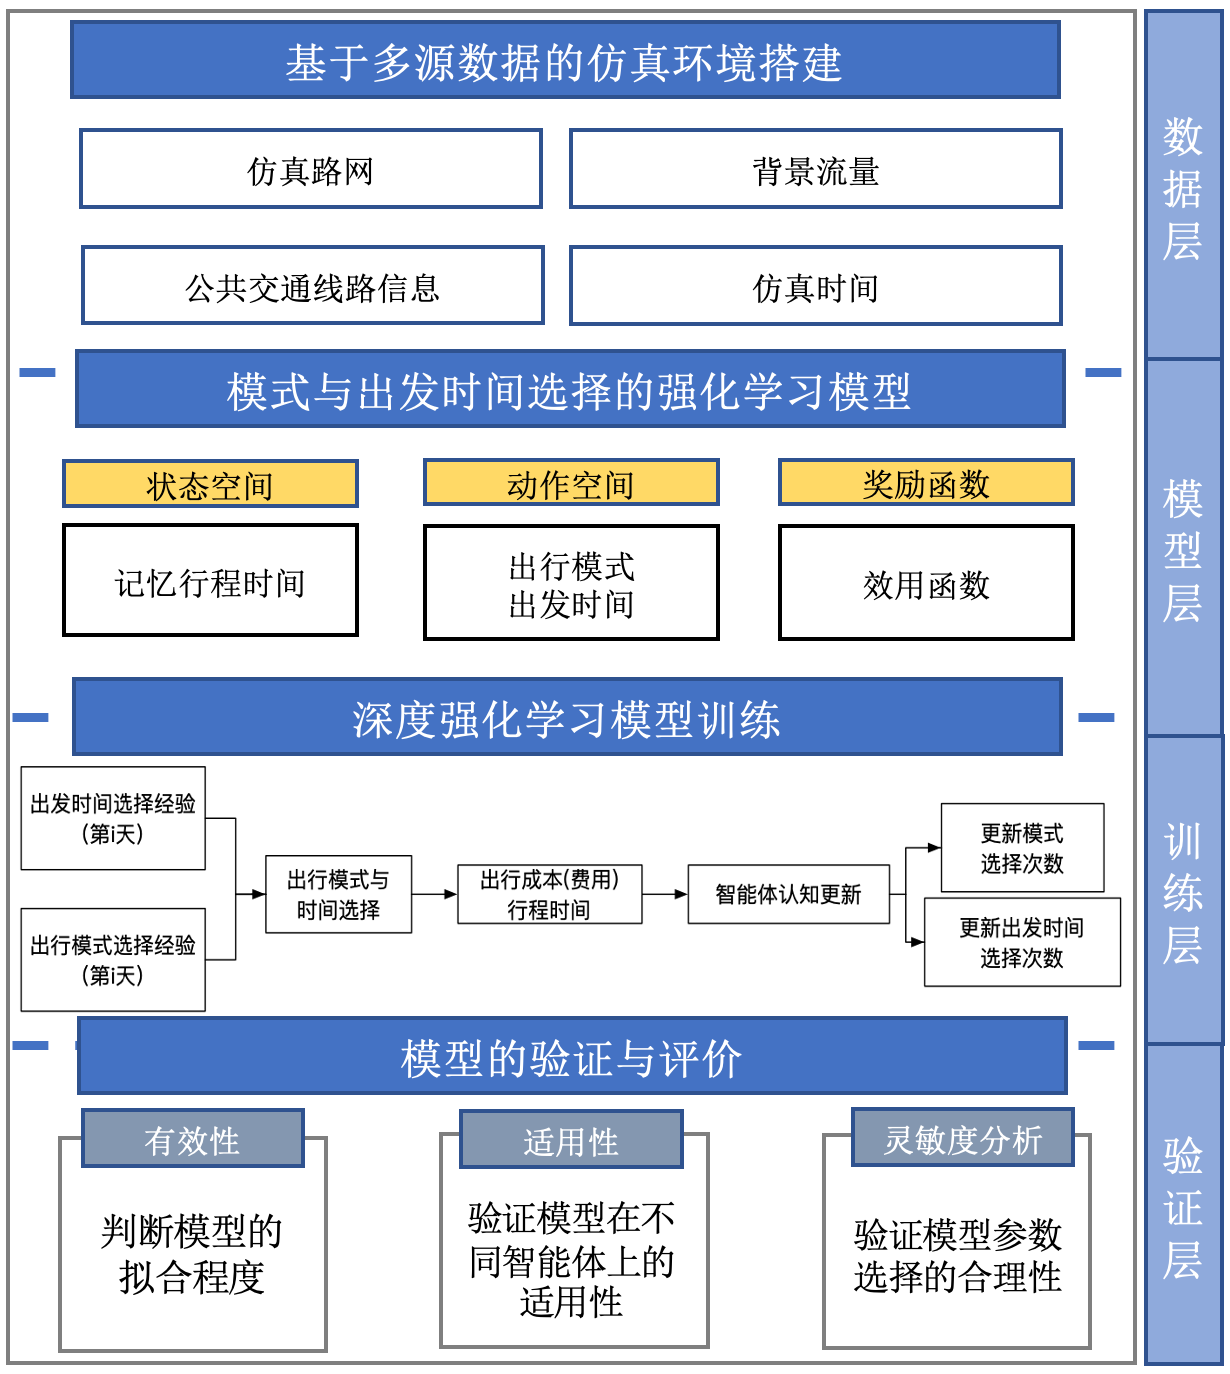
\includegraphics[width=0.92\linewidth]{figures/content/flowchart.png}
  \caption{技术路线图}
  \label{flowchart}
\end{figure}